\chapter{Plans for the next semester} \label{future_plans}

In this chapter we are going to review the plans for the next semester.

\section{Hardware architecture}

As we mentioned the camera above the LIDAR is not able to detect humans due to its limited FOV so the architecture of our system should be modified. Our suggestion is to leave the OAK-D Pro in its original position and use another camera (maybe the OAK-D which I used for experiments at home) at the front, tilted upwards. The OAK-D Pro would be responsible for the visual mapping and the other one would perform the person detection. Of course it is going to take some time to appropriately implement the positioning and mounting of the camera but we agree that it could be a profitable solution. Furthermore, the detector camera could be connected to the notebook and the detected persons' location could be sent to the robot and/or to the mapping service.

\begin{figure}[H]
    \centering
    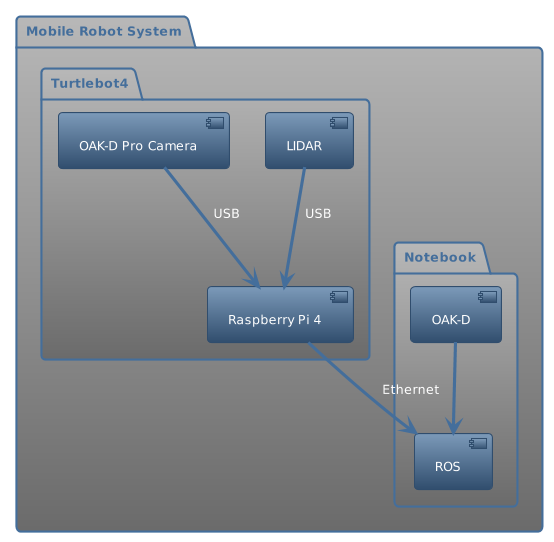
\includegraphics[width=90mm, keepaspectratio]{figures/suggested_architecture.png}
    \caption{Suggested architecture with another camera}
    \label{fig:suggested_architecture}
\end{figure}

\section{Person detection}

In the next semester it is mandatory to create a well-functioning person detector so the robot could be able to follow or avoid people near itself.

\section{Mapping}

Our goal is to find a solution for the mapping because RTAB-Map had several problems which cannot be resolved easily. Fortunately we have several ideas:

\begin{itemize}
    \item Create a mapping tool with the Spectacular AI SDK (the examples showed great performance and results with the camera)
    \item We could use nvblox to construct maps\footnote{\url{https://nvblox.readthedocs.io/en/latest/}}
\end{itemize}

\section{Localization}

After we created a map it would be interesting to try out several approaches of photorealistic localisation. We could train NeRFs or create Gaussian Splats from the mapped environment and then use a tool that can navigate the robot in the splat or NeRF map. Some tools we could try:
\begin{itemize}
    \item NerfNavigation\footnote{\url{https://mikh3x4.github.io/nerf-navigation/}}
    \item SplatNav\cite{splatnav}
    \item SplaTAM\cite{splatam}
    \item And a lot more...\cite{nerf_robotics_cites}
\end{itemize}
